\section{Pregunta N$^{\circ}$7\qquad León Alonzo Terrones Caccha}

\begin{frame}
	\frametitle{Interpolación polinomial}

	\begin{definition}[Conjunto nodal]
		Sea
		\begin{math}
			\left[a,b\right]\subset
			\mathbb{R}
		\end{math}.
		$T$ es un \alert{conjunto nodal} de tamaño
		$n+1\in\mathbb{N}$ en $\left[a,b\right]$ sii
		\begin{math}
			T=
			{
			\left\{
			t_{i}
			\right\}
			}^{n}_{i=0}\subset
			\left[a,b\right]
		\end{math}
		es un conjunto de elementos distintos.
		Los elementos de $T$, $t_{i}$ son llamados \alert{nodos}.
	\end{definition}

	\begin{definition}[Polinomio interpolante]
		Sean
		\begin{math}
			T=
			{
			\left\{
			t_{i}
			\right\}
			}^{n}_{i=0}\subset
			\left[a,b\right]
		\end{math}
		un conjunto nodal y
		\begin{math}
			f\colon
			\left[a,b\right]\to
			\mathbb{R}
		\end{math}
		una función.
		La función $I\colon\left[a,b\right]\to\mathbb{R}$ es llamada un
		\alert{interpolante de} $f$ subordinado a $T$ sii
		\begin{math}
			\forall i\in\left\{0,\dotsc,n\right\}:
			I\left(t_{i}\right)=f\left(t_{i}\right)
		\end{math}.
		En este caso, escribimos
		\begin{math}
			I\left(T\right)=
			f\left(T\right)
		\end{math}.
	\end{definition}

	\begin{definition}[Polinomio de interpolación]
		Sea
		\begin{math}
			X=
			{
			\left\{
			x_{i}
			\right\}
			}^{n}_{i=0}\subset
			\mathbb{R}
		\end{math}
		un conjunto de puntos no necesariamente distintos.
		Defina el conjunto de pares ordenados
		\begin{equation*}
			O\coloneqq
			\left\{
			\left(x_{i},y_{i}\right)\mid
			t_{i}\in T,
			x_{i}\in X,
			\forall i\in\left\{0,\dotsc,n\right\}
			\right\}
		\end{equation*}
		$I$ es un interpolante de $O$ sii
		\begin{math}
			\forall i\in\left\{0,\dotsc,n\right\}:
			I\left(t_{i}\right)=
			f\left(t_{i}\right)
		\end{math},
		es decir, $I\left(T\right)=X$.
		Si el interpolante $I$ es un polinomio, este es llamado un
		\alert{polinomio de interpolación}.
	\end{definition}

	% Sean $n+1$ puntos distintos
	% \begin{math}
	% 	{
	% 		\left\{
	% 		\left(x_{k},y_{k}\right)
	% 		\right\}
	% 	}_{k=0}^{n}\subset
	% 	\left[a,b\right]\times\mathbb{R}
	% \end{math}
	% y
	% \begin{math}
	% 	f\colon\left[a,b\right]\to
	% 	\mathbb{R}
	% \end{math}
	% una función de modo que
	% \begin{math}
	% 	y_{k}=
	% 	f\left(x_{k}\right)
	% \end{math}
	% para $0\leq k\leq n$.

	% Here $\ell_{0},\ell_{1},\ldots,\ell_{n}$ are polynomials that
	% depend on the nodes $x_0, x_1, \ldots, x_n$ but not on the
	% ordinates $y_{0},y_{1},\ldots,y_{n}$.
	% Since all the ordinates could be $0$ except for a $1$ occupying the
	% $i$-th position, we see that

	% \begin{equation*}
	% 	\delta_{ij}=
	% 	p_{n}
	% 	\left(x_j\right)=
	% 	\sum\limits_{k=0}^{n}
	% 	y_{k}
	% 	\ell_k\left(x_j\right)=
	% 	\sum\limits_{k=0}^{n}
	% 	\delta_{ki}
	% 	\ell_{k}
	% 	\left(x_j\right)=
	% 	\ell_{i}
	% 	\left(x_j\right).
	% \end{equation*}

	% (Recall that the Kronecker delta is defined by $\delta_{k i}=1$ if
	% $k=i$ and $\delta_{k i}=0$ if $k \neq i$.)
	% We can easily arrive at a set of polynomials having this property.
	% Let us consider $\ell_{0}$.
	% It is to be a polynomial of degree $n$ that takes the value $0$ at
	% $x_{1},x_{2},\ldots,x_{n}$ and the value $1$ at $x_0$.
	% Clearly, $\ell_{0}$ must be of the form

	% \begin{equation*}
	% 	\ell_{0}
	% 	\left(x\right)=
	% 	c
	% 	\left(x-x_1\right)
	% 	\left(x-x_2\right)\cdots
	% 	\left(x-x_n\right)=
	% 	c
	% 	\prod\limits_{j=1}^{n}
	% 	\left(x-x_j\right).
	% \end{equation*}

	% The value of $c$ is obtained by putting $x=x_{0}$, so that
	% \begin{math}
	% 	1=
	% 	c
	% 	\prod\limits_{j=1}^{n}
	% 	\left(x_{0}-x_{j}\right)
	% \end{math}
	% y
	% \begin{math}
	% 	c=
	% 	\prod\limits_{j=1}^{n}
	% 	{\left(x_{0}-x_{j}\right)}^{-1}
	% \end{math}.

	\begin{definition}[Matriz de Vandermonde]
		Sea
		\begin{math}
			T=
			{
			\left\{
			t_{i}
			\right\}
			}^{n}_{i=0}
		\end{math}
		un conjunto nodal.
		La \alert{matriz de Vandermonde} subordinada al conjunto
		nodal $T$, denotada por
		\begin{math}
			V_{n}=
			\left[v_{ij}\right]\in
			\mathbb{R}^{\left(n+1\right)\times\left(n+1\right)}
		\end{math}
		es la matriz con entradas
		\begin{math}
			\forall\left\{i,j\right\}\subset
			\left\{1,\dotsc,n+1\right\}:
			v_{ij}=
			t^{j-1}_{i-1}
		\end{math},
		es decir,
		\begin{equation*}
			V_{n}=
			\begin{bmatrix}
				1      & t_{0} & \cdots & t_{0}^{n} \\
				\vdots & t_{1} & \ddots & \vdots    \\
				1      & t_{n} & \cdots & t_{n}^{n}
			\end{bmatrix}.
		\end{equation*}
	\end{definition}
\end{frame}

\begin{frame}
	\begin{definition}[Operador de interpolación]
		Sea
		\begin{math}
			T=
			{
			\left\{
			t_{i}
			\right\}
			}^{n}_{i=0}
		\end{math}
		un conjunto nodal.
		El \alert{operador de interpolación} subordinado a $T$ es
		\begin{math}
			\mathcal{I}_{T}:
			C\left(\left[a,b\right]\right)\to
			\mathbb{P}_{n}
		\end{math}
		donde
		\begin{math}
			\mathcal{I}_{T}
			\left[f\right]
		\end{math}
		es el único polinomio de interpolación
		que satisface
		\begin{math}
			\mathcal{I}_{T}
			\left[f\right]
			\left(T\right)=
			f\left(T\right)
		\end{math}.
	\end{definition}

	\begin{theorem}[Operador de proyección lineal]
		Sea
		\begin{math}
			T=
			{
			\left\{
			t_{i}
			\right\}
			}^{n}_{i=0}
			\subset\left[a,b\right]
		\end{math}
		un conjunto nodal e
		\begin{math}
			\mathcal{I}_{T}:
			C\left(\left[a,b\right]\right)\to
			\mathbb{P}_{n}
		\end{math}
		es el operador de interpolación subordinado a $T$.
		\begin{math}
			\mathcal{I}_{T}
		\end{math}
		es un \alert{operador de proyección lineal} sii
		\begin{equation*}
			\forall f,g\in C\left(\left[a,b\right]\right):
			\forall\alpha\in\mathbb{R}:
			\mathcal{I}_{T}\left[\alpha f+g\right]=
			\alpha\mathcal{I}_{T}\left[f\right]+
			\mathcal{I}_{T}\left[g\right],\qquad
			\forall p\in\mathbb{P}_{n}:
			\mathcal{I}_{T}\left[p\right]=
			p.
		\end{equation*}
	\end{theorem}

	\begin{definition}[Constante de Lebesgue]
		Sea
		\begin{math}
			T=
			{
			\left\{
			t_{i}
			\right\}
			}^{n}_{i=0}
			\subset\left[a,b\right]
		\end{math}
		un conjunto nodal e
		\begin{math}
			\mathcal{I}_{T}:
			C\left(\left[a,b\right]\right)\to
			\mathbb{P}_{n}
		\end{math}
		es el operador de interpolación subordinado a $T$.
		La \alert{constante de Lebesgue subordinada a} $T$,
		$\Lambda\left(T\right)$, es la norma del operador
		$\mathcal{I}_{T}$, es
		decir,
		\begin{math}
			\Lambda\left(T\right)=
			{\left\|
			\mathcal{I}_{T}
			\right\|}_{\infty}
		\end{math},
		donde
		\begin{equation*}
			{\left\|
				\mathcal{I}_{T}
				\right\|}_{\infty}=
			\sup_{f\neq0}
			\dfrac{
				{\left\|
						\mathcal{I}_{T}
						\left[f\right]
						\right\|}_{\infty}
			}{
				{\left\|f\right\|}_{\infty}
			}=
			\sup_{
				{\left\|f\right\|}_{\infty}=1}
			\left\|
			\mathcal{I}_{T}
			\left[f\right]
			\right\|_{\infty}.
		\end{equation*}
	\end{definition}
\end{frame}

\begin{frame}
	\begin{definition}[Polinomio de interpolación en la forma de Lagrange]
		Sea
		\begin{math}
			T=
			{
			\left\{
			t_{i}
			\right\}
			}^{n}_{i=0}
			\subset\left[a,b\right]
		\end{math}
		un conjunto nodal.
		El \alert{polinomio de interpolación de Lagrange} de la función $f$,
		subordinada al conjunto nodal $T$, es el polinomio
		\begin{equation*}
			\Pi_{n}
			f\left(t\right)\coloneqq
			% y_{0}
			% \ell_{0}\left(x\right)+
			% y_{1}
			% \ell_{1}\left(x\right)+
			% \cdots+
			% y_{n}
			% \ell_{n}\left(x\right)=
			\sum\limits_{k=0}^{n}
			x_{k}
			\ell_{k}\left(t\right)\in\mathbb{P}_{n},
		\end{equation*}
		donde
		\begin{math}
			\ell_{k}
			\left(t\right)\coloneqq
			\prod\limits_{\substack{j=0\\j\neq k}}^{n}
			\dfrac{t-t_{j}}{t_{k}-t_{j}}
		\end{math}
		para $0\leq k\leq n$ son las \alert{bases nodales de Lagrange}
		que satisface
		\begin{math}
			\ell_{k}
			\left(t_{j}\right)=
			\delta_{kj}
		\end{math}.

		La evaluación de $\Pi_{n}f\left(t\right)$ requiere
		$O\left(n^{2}\right)$ sumas y productos, en general el
		algoritmo es \emph{numéricamente inestable}.
	\end{definition}

	\begin{definition}[Polinomio de interpolación en la forma de Newton]
		\begin{equation*}
			\Pi_{n}
			f\left(t\right)\coloneqq
			\sum\limits_{k=0}^{n}
			a_{k}
			\omega_{k}\left(t\right)\in\mathbb{P}_{n},
		\end{equation*}
		donde
		\begin{itemize}
			\item

			      \begin{math}
				      a_{k}\coloneqq
				      f\left[t_{0},\ldots,t_{k}\right]
			      \end{math}
			      es la \alert{$k$-ésima diferencia dividida de Newton}, y

			\item

			      \begin{math}
				      \omega_{k}
				      \left(t\right)\coloneqq
				      \prod\limits_{j=0}^{k-1}
				      \left(
				      t-t_{j}
				      \right)
			      \end{math}
			      es el \alert{polinomio nodal de grado $k$}.
		\end{itemize}
		La evaluación de $\Pi_{n}f\left(t\right)$ requiere
		$O\left(n\right)$.
	\end{definition}
\end{frame}

% https://people.maths.ox.ac.uk/trefethen/barycentric.pdf
% \begin{frame}
% 	\begin{definition}[Interpolación baricéntrica de Lagrange]
% 		Con el fin de realizar menos operaciones en la interpolación
% 		polinomial de Lagrange, multiplicamos por
% 		\begin{math}
% 			\alert{
% 				\dfrac{1}{\omega_{n+1}\left(x\right)}
% 			}
% 		\end{math}
% 		y resulta
% 		\begin{align*}
% 			\alert{
% 				\dfrac{1}{\omega_{n+1}\left(x\right)}
% 			}
% 			\Pi_{n}f\left(x\right) & =
% 			\alert{
% 				\dfrac{1}{\omega_{n+1}\left(x\right)}
% 			}
% 			\sum\limits_{k=0}^{n}
% 			y_{k}
% 			\alert{
% 				\ell_{k}\left(x\right)
% 			}=
% 			\dfrac{1}{\omega_{n+1}\left(x\right)}
% 			\sum\limits_{k=0}^{n}
% 			y_{k}
% 			\alert{
% 			\prod\limits_{\substack{j=0 \\j\neq k}}^{n}
% 			\dfrac{x-x_{j}}{x_{k}-x_{j}}
% 			}.
% 			\\
% 			                       & =
% 			\sum\limits_{k=0}^{n}
% 			\left\{
% 			\dfrac{y_{k}}{
% 				\alert{
% 			\prod\limits_{\substack{j=0 \\j\neq k}}^{n}
% 					\left(
% 					x_{k}-x_{j}
% 					\right)
% 				}
% 			}
% 			\dfrac{
% 				\alert{
% 			\prod\limits_{\substack{j=0 \\j\neq k}}^{n}
% 					\left(
% 					x-x_{j}
% 					\right)
% 				}
% 			}{\omega_{n+1}\left(x\right)}
% 			\right\}=
% 			\sum\limits_{k=0}^{n}
% 			\left\{
% 			\dfrac{y_{k}}{
% 			\prod\limits_{\substack{j=0 \\j\neq k}}^{n}
% 				\left(
% 				x_{k}-x_{j}
% 				\right)
% 			}
% 			\dfrac{1}{x-x_{k}}
% 			\right\}.
% 			\\
% 			\Pi_{n}f\left(x\right)
% 			                       & =
% 			\sum\limits_{k=0}^{n}
% 			y_{k}
% 			\widetilde{\ell}_{k}\left(x\right)\in\mathbb{P}_{n},
% 		\end{align*}
% 		donde
% 		\begin{columns}
% 			\begin{column}{.45\paperwidth}
% 				\begin{itemize}
% 					\item

% 					      \begin{math}
% 						      \widetilde{\ell}_{k}
% 						      \left(x\right)=
% 						      \omega_{n+1}
% 						      \left(x\right)
% 						      \dfrac{b_{k}}{x-x_{k}}
% 					      \end{math}, y
% 				\end{itemize}
% 			\end{column}
% 			\begin{column}{.45\paperwidth}
% 				\begin{itemize}
% 					\item

% 					      \begin{math}
% 						      b_{j}=
% 						      \dfrac{1}{
% 							      \prod\limits_{\substack{j=0\\j\neq k}}^{n}
% 							      \left(
% 							      x_{k}-x_{j}
% 							      \right)
% 						      }
% 					      \end{math}
% 					      son los \emph{pesos baricéntricos}.
% 				\end{itemize}
% 			\end{column}
% 		\end{columns}
% 		% La evaluación de $\Pi_{n}f\left(x\right)$ requiere
% 		% $O\left(n\right)$.
% 	\end{definition}
% \end{frame}
% \begin{frame}
	\begin{theorem}
		Para $0\leq k\leq n$ se cumple
		\begin{math}
			\omega^{\prime}_{n+1}
			\left(x_{k}\right)=
			\prod\limits_{\substack{j=0\\j\neq k}}^{n}
			\left(
			x_{k}-x_{j}
			\right).
		\end{math}
	\end{theorem}

	\begin{proof}
		Si
		\begin{math}
			\omega_{\alert{n+1}}
			\left(x\right)
			\overset{\text{def}}{=}
			\prod\limits_{j=0}^{\alert{n+1}-1}
			\left(
			x-x_{j}
			\right)=
			\prod\limits_{j=0}^{n}
			\left(
			x-x_{j}
			\right)
		\end{math}, entonces
		\begin{math}
			\ln
			\left(
			\omega_{n+1}
			\left(x\right)
			\right)=
			\ln
			\left(
			\prod\limits_{j=0}^{n}
			\left(
				x-x_{j}
				\right)
			\right)=
			\sum\limits_{j=0}^{n}
			\ln
			\left(
			x-x_{j}
			\right)
		\end{math}.
		Derivando,

		\begin{align*}
			{\left(
				\ln
				\left(
					\omega_{n+1}
					\left(x\right)
					\right)
			\right)}^{\prime} & =
			{\left(
			\sum\limits_{j=0}^{n}
			\ln
			\left(
				x-x_{j}
				\right)
			\right)}^{\prime}=
			\sum\limits_{j=0}^{n}
			{\left(
			\ln
			\left(
				x-x_{j}
				\right)
			\right)}^{\prime}.
			\\
			\dfrac{
				\omega^{\prime}_{n+1}\left(x\right)
			}{
				\alert{
					\omega_{n+1}\left(x\right)
				}
			}                 & =
			\sum\limits_{j=0}^{n}
			\dfrac{{\left(x-x_{j}\right)}^{\prime}}{x-x_{j}}=
			\sum\limits_{j=0}^{n}
			\dfrac{1}{x-x_{j}}.
			\\
			\Aboxed{
			w^{\prime}_{n+1}
			\left(x\right)    & =
			\alert{
				\omega_{n+1}
				\left(x\right)
			}
			\sum\limits_{j=0}^{n}
			\dfrac{1}{x-x_{j}}.
			}
			\\
			w^{\prime}_{n+1}
			\left(x_{k}\right)
			                  & =
			\alert{
				\prod\limits_{j=0}^{n}
				\left(
				x_{k}-x_{j}
				\right)
			}
			\sum\limits_{i=0}^{n}
			\dfrac{1}{x_{k}-x_{i}}=
			\prod\limits_{j=0}^{n}
			\sum\limits_{i=0}^{n}
			\dfrac{
			x_{k}-x_{j}
			}{
			x_{k}-x_{i}
			}
			=
			\prod\limits_{\substack{j=0 \\j\neq k}}^{n}
			\left(
			x_{k}-x_{j}
			\right).
		\end{align*}
		% Si $x_{k}$ un punto nodal cualesquiera, donde $0\leq k\leq n$,
		% entonces
		% \begin{math}
		% 	w^{\prime}_{n+1}
		% 	\left(x_{k}\right)=
		% 	\prod\limits_{\substack{j=0 \\j\neq k}}^{n}
		% 	\left(
		% 	x_{k}-x_{j}
		% 	\right)
		% \end{math}.
	\end{proof}
\end{frame}

\begin{frame}
	\begin{theorem}
		Si $\Pi_{n}f\left(x\right)$ es el polinomio de Lagrange, entonces
		\begin{math}
			\Pi_{n}f\left(x\right)=
			\sum\limits_{k=0}^{n}
			\dfrac{
				\omega_{n+1}\left(x\right)
			}{
				\left(x-x_{k}\right)
				\omega^{\prime}_{n+1}\left(x_{k}\right)
			}
			y_{k}
		\end{math}.
	\end{theorem}

	\begin{proof}
		\begin{align*}
			\sum\limits_{k=0}^{n}
			\dfrac{
				\omega_{n+1}\left(x\right)
			}{
				\left(x-x_{k}\right)
				\alert{
					\omega^{\prime}_{n+1}\left(x_{k}\right)
				}
			}
			y_{k} & =
			\sum\limits_{k=0}^{n}
			y_{k}
			\dfrac{
				\prod\limits_{j=0}^{n}
				\left(
				x-x_{j}
				\right)
			}{
				\left(x-x_{k}\right)
				\alert{
			\prod\limits_{\substack{j=0 \\j\neq k}}^{n}
					\left(
					x_{k}-x_{j}
					\right)
				}
			}
			\\
			      & =
			\sum\limits_{k=0}^{n}
			y_{k}
			\dfrac{
			\prod\limits_{\substack{j=0 \\j\neq k}}^{n}
				\left(
				x-x_{j}
				\right)
			}{
			\prod\limits_{\substack{j=0 \\j\neq k}}^{n}
				\left(
				x_{k}-x_{j}
				\right)
			}
			\\
			      & =
			\sum\limits_{k=0}^{n}
			y_{k}
			\alert{
			\prod\limits_{\substack{j=0 \\j\neq k}}^{n}
			\dfrac{
			x-x_{j}
			}{
			x_{k}-x_{j}
			}
			}                           \\
			      & =
			\sum\limits_{k=0}^{n}
			y_{k}
			\alert{
				\ell_{k}\left(x\right)
			}
			=
			\Pi_{n}
			f\left(x\right).
		\end{align*}
	\end{proof}
\end{frame}

\begin{frame}
	\begin{theorem}[Teorema de las diferencias divididas de orden superior]
		Para $0\leq k\leq n$ se cumple
		\begin{equation*}
			a_{k}=
			f\left[x_{0},\ldots,x_{k}\right]=
			\dfrac{
			f\left[x_{1},\ldots,x_{k}\right]-
			f\left[x_{0},\ldots,x_{k-1}\right]
			}{x_{k}-x_{0}}.
			% \begin{cases}
			% 	0 & \text{si} \\
			% 	1 & \text{no}
			% \end{cases}
		\end{equation*}
		La evaluación de $a_{n}$ requiere $n^{2}$ restas y
		$\dfrac{n^{2}}{2}$ divisiones.
	\end{theorem}

	% \begin{proof}
	% 	.
	% \end{proof}

	\begin{theorem}[Representación explícita de $a_{n}$]
		¿Encontrar alguna identidad entre $\omega_{k}\left(x\right)$ y
		$\ell_{k}\left(x\right)$?
		\begin{equation*}
			a_{n}=
			\sum\limits_{k=0}^{n}
			\dfrac{
				f\left(x_{k}\right)
			}{
				w^{\prime}_{n+1}
				\left(x_{k}\right)
			}.
		\end{equation*}
	\end{theorem}

	\begin{proof}
		\begin{equation*}
			\sum\limits_{k=0}^{n}
			\dfrac{
				f\left(x_{k}\right)
			}{
				\alert{
					w^{\prime}_{n+1}
					\left(x_{k}\right)
				}
			}=
			\sum\limits_{k=0}^{n}
			\dfrac{
				f\left(x_{k}\right)
			}{
				\alert{
					\prod\limits_{\substack{j=0 \\j\neq k}}^{n}
					\left(
					x_{k}-x_{j}
					\right)
				}
			}
		\end{equation*}
	\end{proof}

	% \begin{theorem}[Interpolación de Lagrange baricéntrica] % Fórmula baricéntrica
	% 	\begin{equation*}
	% 		\lambda_{k}\coloneqq
	% 		\prod\limits_{\substack{j=0               \\j\neq k}}^{n}
	% 		\dfrac{1}{x_{k}-x_{j}}=
	% 		\dfrac{1}{\prod\limits_{\substack{j=0               \\j\neq k}}^{n}x_{k}-x_{j}}
	% 	\end{equation*}
	% \end{theorem}
\end{frame}

\begin{frame}
	\begin{enumerate}\setcounter{enumi}{5}
		\item

		      Encuentre el interpolante de Lagrange
		      \begin{math}
			      p_{3}\left(t\right)=
			      \sum\limits_{k=0}^{3}
			      x_{k}
			      \ell_{k}\left(t\right)
		      \end{math}
		      para el conjunto de datos
		      \begin{math}
			      \left\{
			      \left(0,1\right),
			      \left(\frac{1}{2},2\right),
			      \left((1,\frac{3}{2}\right),
                    \left((2,-1\right)
			      \right\}
		      \end{math}.
		      Encuentre $p_{2,k}$ en
		      \begin{math}
			      p_{3}\left(t\right)=
			      \sum\limits_{k=0}^{3}
			      p_{3,k}t^{k}
		      \end{math}.
	\end{enumerate}

	\begin{solution}
		\begin{align*}
			\ell_{0}\left(t\right) & =
			\prod\limits_{\substack{j=0        \\j\neq 0}}^{n}
			\dfrac{t-t_{j}}{t_{0}-t_{j}}=
			\dfrac{\left(t-t_{1}\right)\left(t-t_{2}\right)}{\left(t_{0}-t_{1}\right)\left(t_{0}-t_{2}\right)}=
			\dfrac{\left(t-0\right)\left(t-1\right)}{\left(\left(-1\right)-0\right)\left(\left(-1\right)-1\right)}=
			\dfrac{1}{2}t\left(t-1\right).     \\
			\ell_{1}\left(t\right) & =
			\prod\limits_{\substack{j=0        \\j\neq 1}}^{n}
			\dfrac{t-t_{j}}{t_{1}-t_{j}}=
			\dfrac{\left(t-t_{0}\right)\left(t-t_{2}\right)}{\left(t_{1}-t_{0}\right)\left(t_{1}-t_{2}\right)}=
			\dfrac{\left(t-\left(-1\right)\right)\left(t-1\right)}{\left(0-\left(-1\right)\right)\left(0-1\right)}=
			-\left(t+1\right)\left(t-1\right). \\
			\ell_{2}\left(t\right) & =
			\prod\limits_{\substack{j=0        \\j\neq 2}}^{n}
			\dfrac{t-t_{j}}{t_{2}-t_{j}}=
			\dfrac{\left(t-t_{0}\right)\left(t-t_{1}\right)}{\left(t_{2}-t_{0}\right)\left(t_{2}-t_{1}\right)}=
			\dfrac{\left(t-\left(-1\right)\right)\left(t-0\right)}{\left(1-\left(-1\right)\right)\left(1-0\right)}=
			\dfrac{1}{2}\left(t+1\right)t.   \\
            \ell_{3}\left(t\right) & =
			\prod\limits_{\substack{j=0        \\j\neq 3}}^{n}
			\dfrac{t-t_{j}}{t_{0}-t_{j}}=
			\dfrac{\left(t-t_{1}\right)\left(t-t_{2}\right)}{\left(t_{0}-t_{1}\right)\left(t_{0}-t_{2}\right)}=
			\dfrac{\left(t-0\right)\left(t-1\right)}{\left(\left(-1\right)-0\right)\left(\left(-1\right)-1\right)}=
			\dfrac{1}{2}t\left(t-1\right).     
		\end{align*}

		Entonces,
		\begin{align*}
			p_{2}\left(t\right) & =
			\sum\limits_{k=0}^{2}
			x_{k}
			\ell_{k}\left(t\right)=
			\alert{x_{0}}\ell_{0}\left(t\right)+
			\alert{x_{1}}\ell_{1}\left(t\right)+
			\alert{x_{2}}\ell_{2}\left(t\right)=
			\dfrac{1}{2}\ell_{0}\left(t\right)+
			\ell_{1}\left(t\right)-
			\ell_{2}\left(t\right).               \\
			                    & =
			\dfrac{1}{2}\alert{\dfrac{1}{2}t\left(t-1\right)}
			\alert{-\left(t+1\right)\left(t-1\right)}-
			\alert{\dfrac{1}{2}\left(t+1\right)t}. \\
			                    & =
			-1.25t^{2}-0.75t+1.
		\end{align*}
	\end{solution}
\end{frame}

\begin{frame}
	\begin{solution}
		\begin{figure}[ht!]
			\centering
			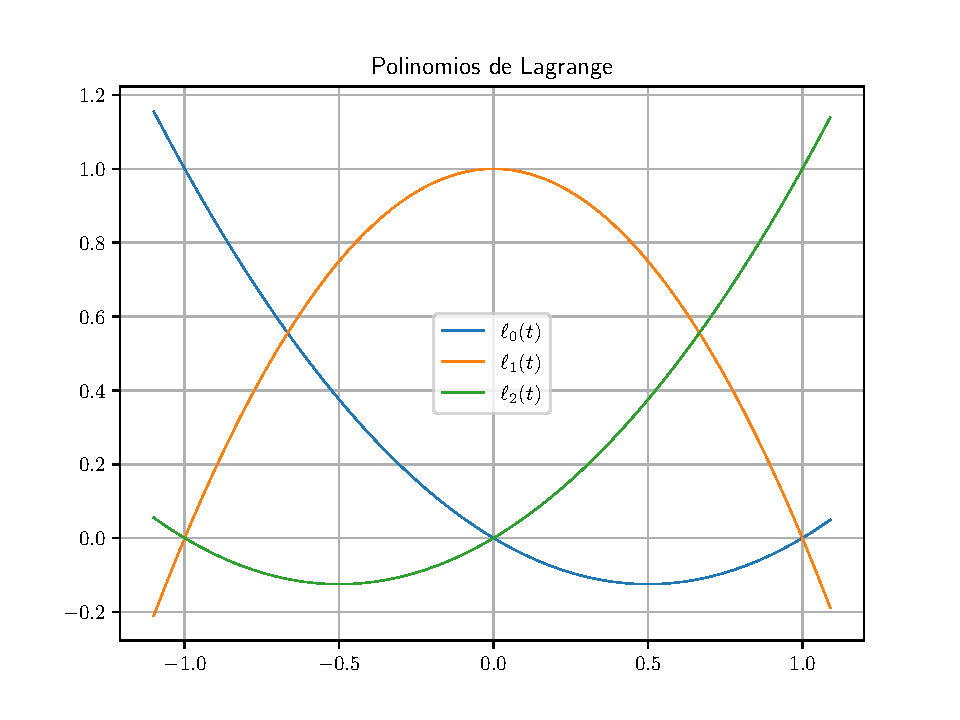
\includegraphics[width=.8\paperwidth]{p6_lagrange}
		\end{figure}
	\end{solution}
\end{frame}


\begin{frame}
	\begin{solution}
		\begin{figure}[ht!]
			\centering
			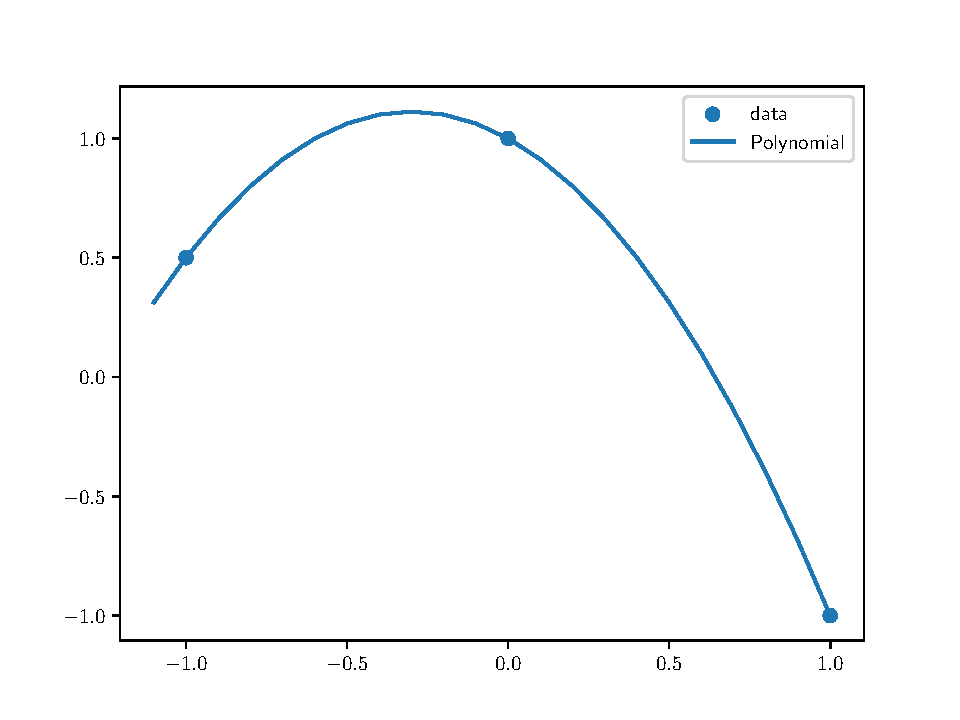
\includegraphics[width=.8\paperwidth]{p6}
		\end{figure}
	\end{solution}
\end{frame}